\documentclass[11pt,a4paper,ngerman]{article}
\usepackage[bottom=2.5cm,top=2.5cm]{geometry} 
\usepackage{babel}
\usepackage[utf8]{inputenc} 
\usepackage[T1]{fontenc} 
\usepackage{ae} 
\usepackage{amssymb} 
\usepackage{amsmath}
\usepackage{amsthm} 
\usepackage{graphicx}
\usepackage{fancyhdr}
\usepackage{caption}
\usepackage{subcaption}
\usepackage{fancyref}
\usepackage{enumerate}
\usepackage{listings}
\usepackage{xcolor}
\usepackage{paralist}
\usepackage{tabularx}

\usepackage[pdftex, bookmarks=false, pdfstartview={FitH}, linkbordercolor=white]{hyperref}
\usepackage{fancyhdr}
\pagestyle{fancy}
\fancyhead[C]{Numerik I}
\fancyhead[L]{Übung 8}
\fancyhead[R]{SoSe 2013}
\fancyfoot{}
\fancyfoot[L]{}
\fancyfoot[C]{\thepage \hspace{1px} of \pageref{LastPage}}
\renewcommand{\footrulewidth}{0.5pt}
\renewcommand{\headrulewidth}{0.5pt}
\setlength{\parindent}{0pt} 
\setlength{\headheight}{0pt}

\date{Tutor: Christina Schulz}
\title{Übung 8}
\author{Max Wisniewski, Alexander Steen}


%%
%% Enviroments for proofs and lemmas
%%
\newtheorem{lemma}{\bfseries Claim}

\begin{document}

\lstset{language=Pascal, basicstyle=\ttfamily\fontsize{10pt}{10pt}\selectfont\upshape, commentstyle=\rmfamily\slshape, keywordstyle=\rmfamily\bfseries, breaklines=true, frame=single, xleftmargin=3mm, xrightmargin=3mm, tabsize=2, mathescape=true}

\renewcommand{\figurename}{Figure}

\maketitle
\thispagestyle{fancy}

%%%%%%%%%%%%%%%%%%%%%%%%%%%%%%
%% Aufgabe 1     %%%%%%%%%%%%%%%%
%%%%%%%%%%%%%%%%%%%%%%%%%%%%%%
\subsection*{Aufgabe 1}
Das Listing~\ref{alg:romberg} zeigt unsere Implementierung der klassichen Romberg-Quadratur.
Bei Eingabe der Integrationsgrenzen, der Funktion und der Liste von Gitterbreiten, wird (wie 
im Skript gezeigt) nach dem Aitken-Neville-Schema die Extrapolation berechnet.
Der Aufruf von \texttt{trapQuad} in der Funktion ist eine leicht modifizierte Version der Funktion vom letzten Übungszettel. Hier wird nicht mehr die Gitterbreite und der Start- und Endpunkt übergeben, sondern das Gittern selber (macht den Code kürzer).

\begin{lstlisting}[language=matlab, numbers=left, caption=Klassische Romberg-Quadratur, label=alg:romberg]
function [S] = romberg(a,b,f,h)
% Gibt den Zahlenwert S der klassischen
% Romberg-Quadratur zurueck
%
% [a,b] Integrationsintervall
% f zu intigrierende Funktion
% h Liste der Schrittweiten
%  (absteigende Gitterbreite!)

% Anzahl der Gitterbreiten
n = length(h);

t = zeros(n,1);

%% Berechnung nach Aitken-Neville-Schema
%% mit Rekursion aus dem Skript
for i = 1:n
  %% summierte Trapezregel zur breite h_i
  t(i) = trapQuad([a:h(i):b],f);
  %% Rekursion
  for k = (i-1):-1:1
    t(k) = t(k+1) + (t(k+1)-t(k))/((h(k)/h(i))^2 - 1);
  end
end
S = t(1);
\end{lstlisting}

Der Test der Funktion wurde wie folgt durchgeführt (Kommentare im Listing).

\begin{lstlisting}[language=matlab,numbers=left]
%% f1 und f2 sind die beiden zu integrierenden Funktionen
f1 = @(x) 1/(2*atan(1)) * 1/(1+x^2);
f2 = @(x) 500/(2*atan(500)) * 1/(1+(500*x)^2);
%% 12x2 Matrizen zur Speicherung der Ergebnisse
%% beider Methoden bei Eingabe f1 bzw. f2
rombergQuad = zeros(12,2);
trapezQuad = zeros(12,2);
%% 12x2 Matrizen der absoluten Fehler
%% beider Methoden
fehlerRomberg = zeros(12,2);
fehlerTrapez = zeros(12,2);
%% Berechnung der Quadratur und Fehler
for i = 1:12
  trapezQuad(i,1) = trapQuad(-1:2^(-i):1,f1);
  trapezQuad(i,2) = trapQuad(-1:2^(-i):1,f2);
  rombergQuad(i,1) = romberg(-1,1,f1,2.^(-[0:i]));
  rombergQuad(i,2) = romberg(-1,1,f2,2.^(-[0:i]));
  fehlerTrapez(i,1) = abs(trapezQuad(i,1) - 1);
  fehlerTrapez(i,2) = abs(trapezQuad(i,2) - 1);
  fehlerRomberg(i,1) = abs(rombergQuad(i,1) - 1);
  fehlerRomberg(i,2) = abs(rombergQuad(i,2) - 1);
end
\end{lstlisting}

Es ergeben sich folgende Fehler (die linke Spalte sind die Fehler von \texttt{f1} ($\gamma = 1$), die rechte Spalte von \texttt{f2} ($\gamma = 500$)). In jeder Spalte ist die $i-te$ Zeile das Ergebnis der Quadratur mit
(feinstem) Gitter $h_i$, $i = 1,.., 12$.
\begin{lstlisting}[basicstyle=\ttfamily\scriptsize\selectfont\upshape]
fehlerTrapez =
   0.013239352830249  78.681790163867319
   0.003315574025695  38.846560808219330
   0.000828929586313  18.935225966615434
   0.000207232961173   8.992119987724385
   0.000051808249116   4.045583465656764
   0.000012952062417   1.621478650708542
   0.000003238015606   0.501227631782829
   0.000000809503901   0.083603568430169
   0.000000202375976   0.003221354221314
   0.000000050593994   0.000005165137005
   0.000000012648499   0.000000000037336
   0.000000003162123   0.000000000012663

fehlerRomberg =
   0.002629023290789  52.122893232379226
   0.000167110611374  23.797834875711604
   0.000002186734143  11.216867628153990
   0.000000003720382   5.114508015192024
   0.000000000015422   2.114728829012008
   0.000000000000023   0.677131955853995
   0.000000000000001   0.068985980824099
   0.000000000000001   0.070952646563530
   0.000000000000001   0.020441181101389
   0.000000000000000   0.000892718805243
   0.000000000000001   0.000059641326506
   0.000000000000002   0.000001316601661
\end{lstlisting}

Der Fehler beider Methoden bei Eingabe von $f$ mit $\gamma = 1$ wird schnell klein; bei der Romberg-Quadratur etwas schneller als bei der summierten Trapezregel. Bei Eingabe von $f$ mit $\gamma = 500$ wird bei beiden Verfahren der Fehler etwas langsamer klein. Im Falle $\gamma = 1$ erzielt die Romberg-Quadratur ein besseres Ergebnis, bei $\gamma = 500$ allerdings die summierte Trapezregel. Figure~\ref{fig:f} zeigt die Graphen von $f$ mit verschiedenem $\gamma$.

\begin{figure}[h!]
\centering
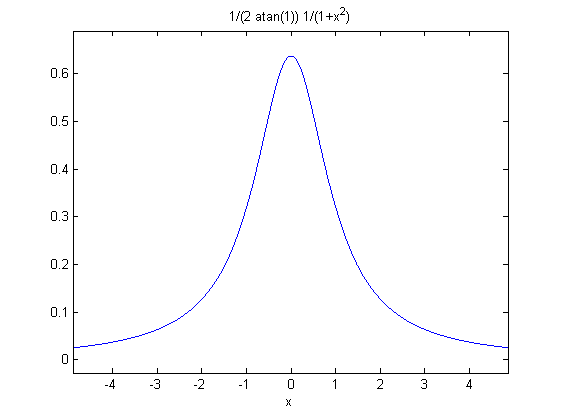
\includegraphics[width=0.48\textwidth]{f1.png}
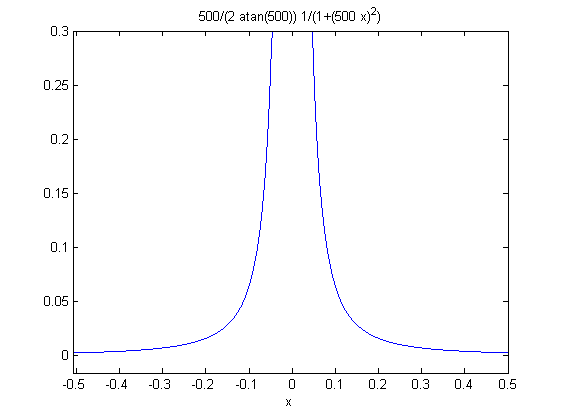
\includegraphics[width=0.48\textwidth]{f2.png}
\caption{Graph der Funktion $f$ mit $\gamma = 1$ (links) und $\gamma = 500$ (rechts) \label{fig:f}}
\end{figure}


%%%%%%%%%%%%%%%%%%%%%%%%%%%%%%
%% Aufgabe 2     %%%%%%%%%%%%%%%%
%%%%%%%%%%%%%%%%%%%%%%%%%%%%%%
\subsection*{Aufgabe 2}

Listing~\ref{lst:adaptiv} zeigt unsere Implementierung der adaptiven Multilevelquadratur in Matlab.
Kommentare sind im Quelltext zu finden.

\begin{lstlisting}[language=matlab,numbers=left,caption=Adaptive Multilevel-Quadratur,label=lst:adaptiv]
function [S] = adapQuad (g, f, tol, n, maxN)

%
% g         - Gitter
% f         - Funktion die zu Integieren ist
%
% tol       - Abstand zwischen Simpson und Trapez
% n         - Schwellwert fuer das verfeinern.
% maxN      - MaxN, maximale Gitterpunkt

m = length(g);

sim = simpQuad(g, f);
trap = trapQuad(g, f);

% Solange wir ueber dem tolleranzwert sind,
% oder wir noch nicht genuegend Stuetzstellen haben
while (abs(sim - trap) > tol) && m < maxN,
    gs = [g(1)];
    %% Unser Schwellwert bezeichnet einen relativen Unterschied zur durchschnittlichen Grenze
    sch = n * (tol / m);
    for k = 2:m,
        %%
        %% Testen wir fuer alle Intervalle, ob wir verfeinern muessen
        %%
        if (abs(simpQuad( g(k-1:k), f) - trapQuad(g(k-1:k), f))) > sch
           gs = [gs ((g(k) + g(k-1))/2) g(k)];
        else
           gs = [gs g(k)]
        end
    end
    g = gs;
    m = length(gs);
    sim = simpQuad(g, f);
    trap = trapQuad(g, f);
end
S = trap;
return
\end{lstlisting}

Wir haben uns für einen Schwellwert entschieden, der den Fehler versucht gleichmäßig auf die Intervalle aufzuteilen. Ist ein Intervall über
dem Durchschnitt (multipliziert mit der Konstante $n$) so halbieren wir es.

Für die Tests wurden alle Zwischenergebnisse mit ausgegeben (das Programm oben also leicht geändert). Es ergeben sich folgende Plots:

\begin{figure}[h!]
\centering
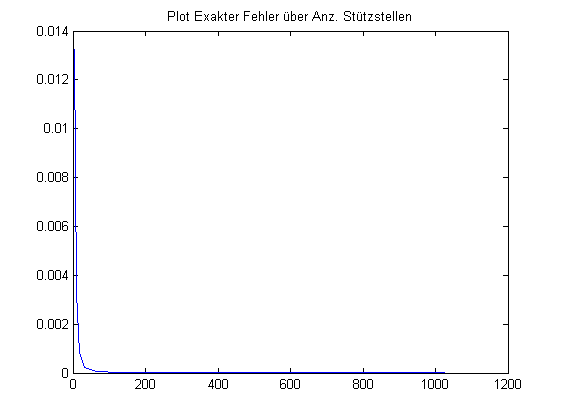
\includegraphics[width=0.48\textwidth]{f1_1.png}
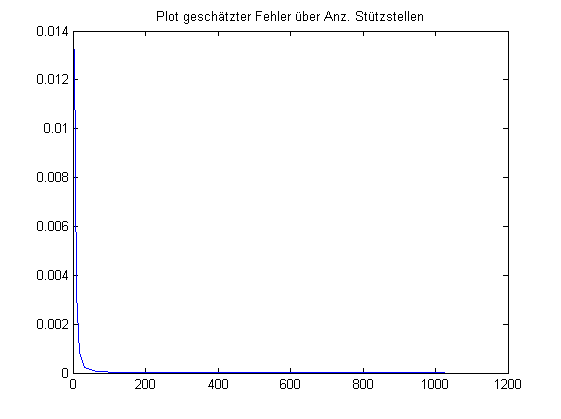
\includegraphics[width=0.48\textwidth]{f1_2.png}
\caption{Graph des exakten Fehlers (links) und geschätzten Fehlers (rechts) über Anz. der Stützstellen mit $\gamma = 1$ \label{fig:f1}}
\end{figure}

\begin{figure}[h!]
\centering
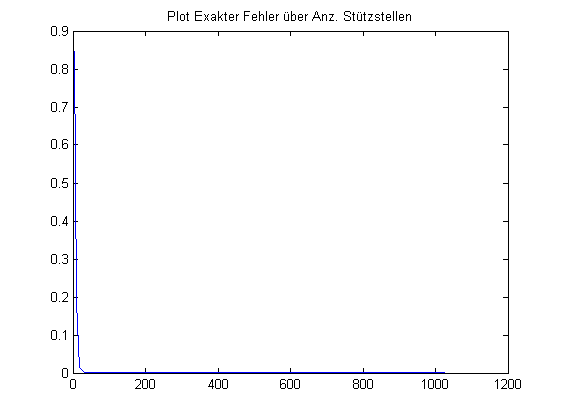
\includegraphics[width=0.48\textwidth]{f2_1.png}
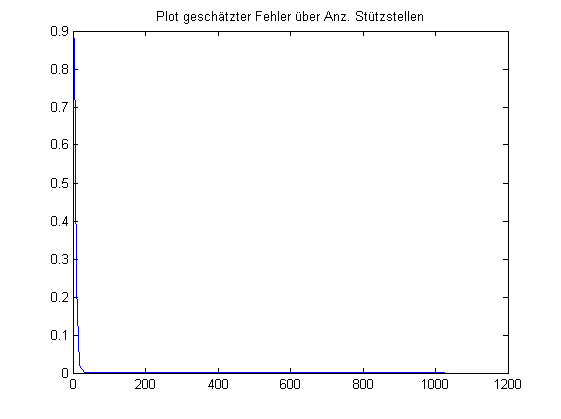
\includegraphics[width=0.48\textwidth]{f2_2.png}
\caption{Graph des exakten Fehlers (links) und geschätzten Fehlers (rechts) über Anz. der Stützstellen mit $\gamma = 10$ \label{fig:f2}}
\end{figure}

\begin{figure}[h!]
\centering
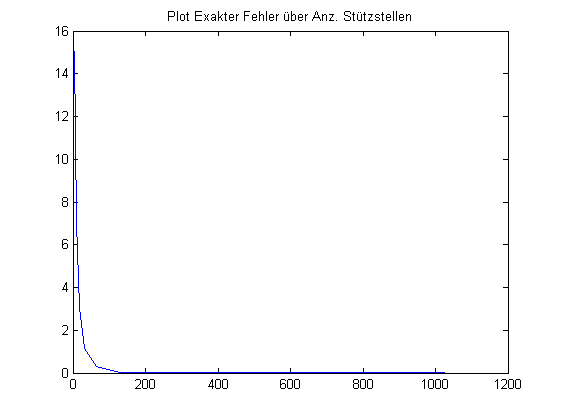
\includegraphics[width=0.48\textwidth]{f3_1.png}
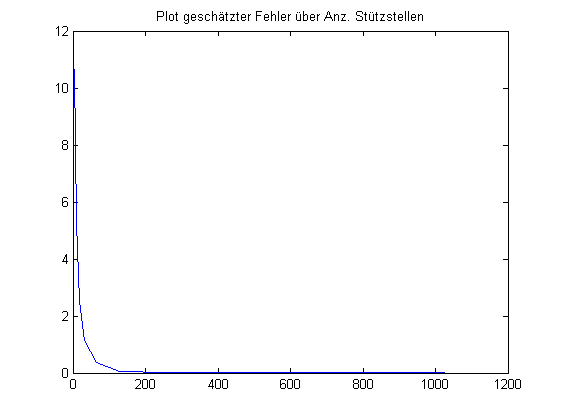
\includegraphics[width=0.48\textwidth]{f3_2.png}
\caption{Graph des exakten Fehlers (links) und geschätzten Fehlers (rechts) über Anz. der Stützstellen mit $\gamma = 100$ \label{fig:f3}}
\end{figure}

Wie wir sehen, sind wir in jedem Test an die Maximalbegrenzung des Gitters gestoßen.\\

Wir haben keine Ahnung, welche Gitterdarstellung sinnvoll sein sollte. Wir konnten beim überfliegen darstellen, dass das Gitter recht nah an
einem Equidistanten lag. Wir wissen nun nicht, ob dies an der Wahl des Schwellwertes lag oder ob der Fehler auf jedem Teilintervall jeweils so groß war,
dass wir verkleinern mussten. Auf jedenfall konnten wir keine Aussagenkräftige darstellung finden (der Plot der Differenz zweier aufeinander folgender Punkte,
sah recht konstant aus).
\newpage
$\quad$
\label{LastPage}
\end{document}
